\section{Number of Effective Queries}

\subsection*{Purpose}

\paragraph{}
To compare the number of effective queries of each sketch under different types of graph streams. 

\paragraph{}
Number of effective queries has been previously defined in the \autoref{section:metrics_neq}. For this experiment, a simple edge query has been selected as the type of the query. If the value of the edge query in the sketch matched the value of the edge query in the original graph, it was considered as an effective query.

\subsection*{Results}

\begin{figure}[H]
    \centering 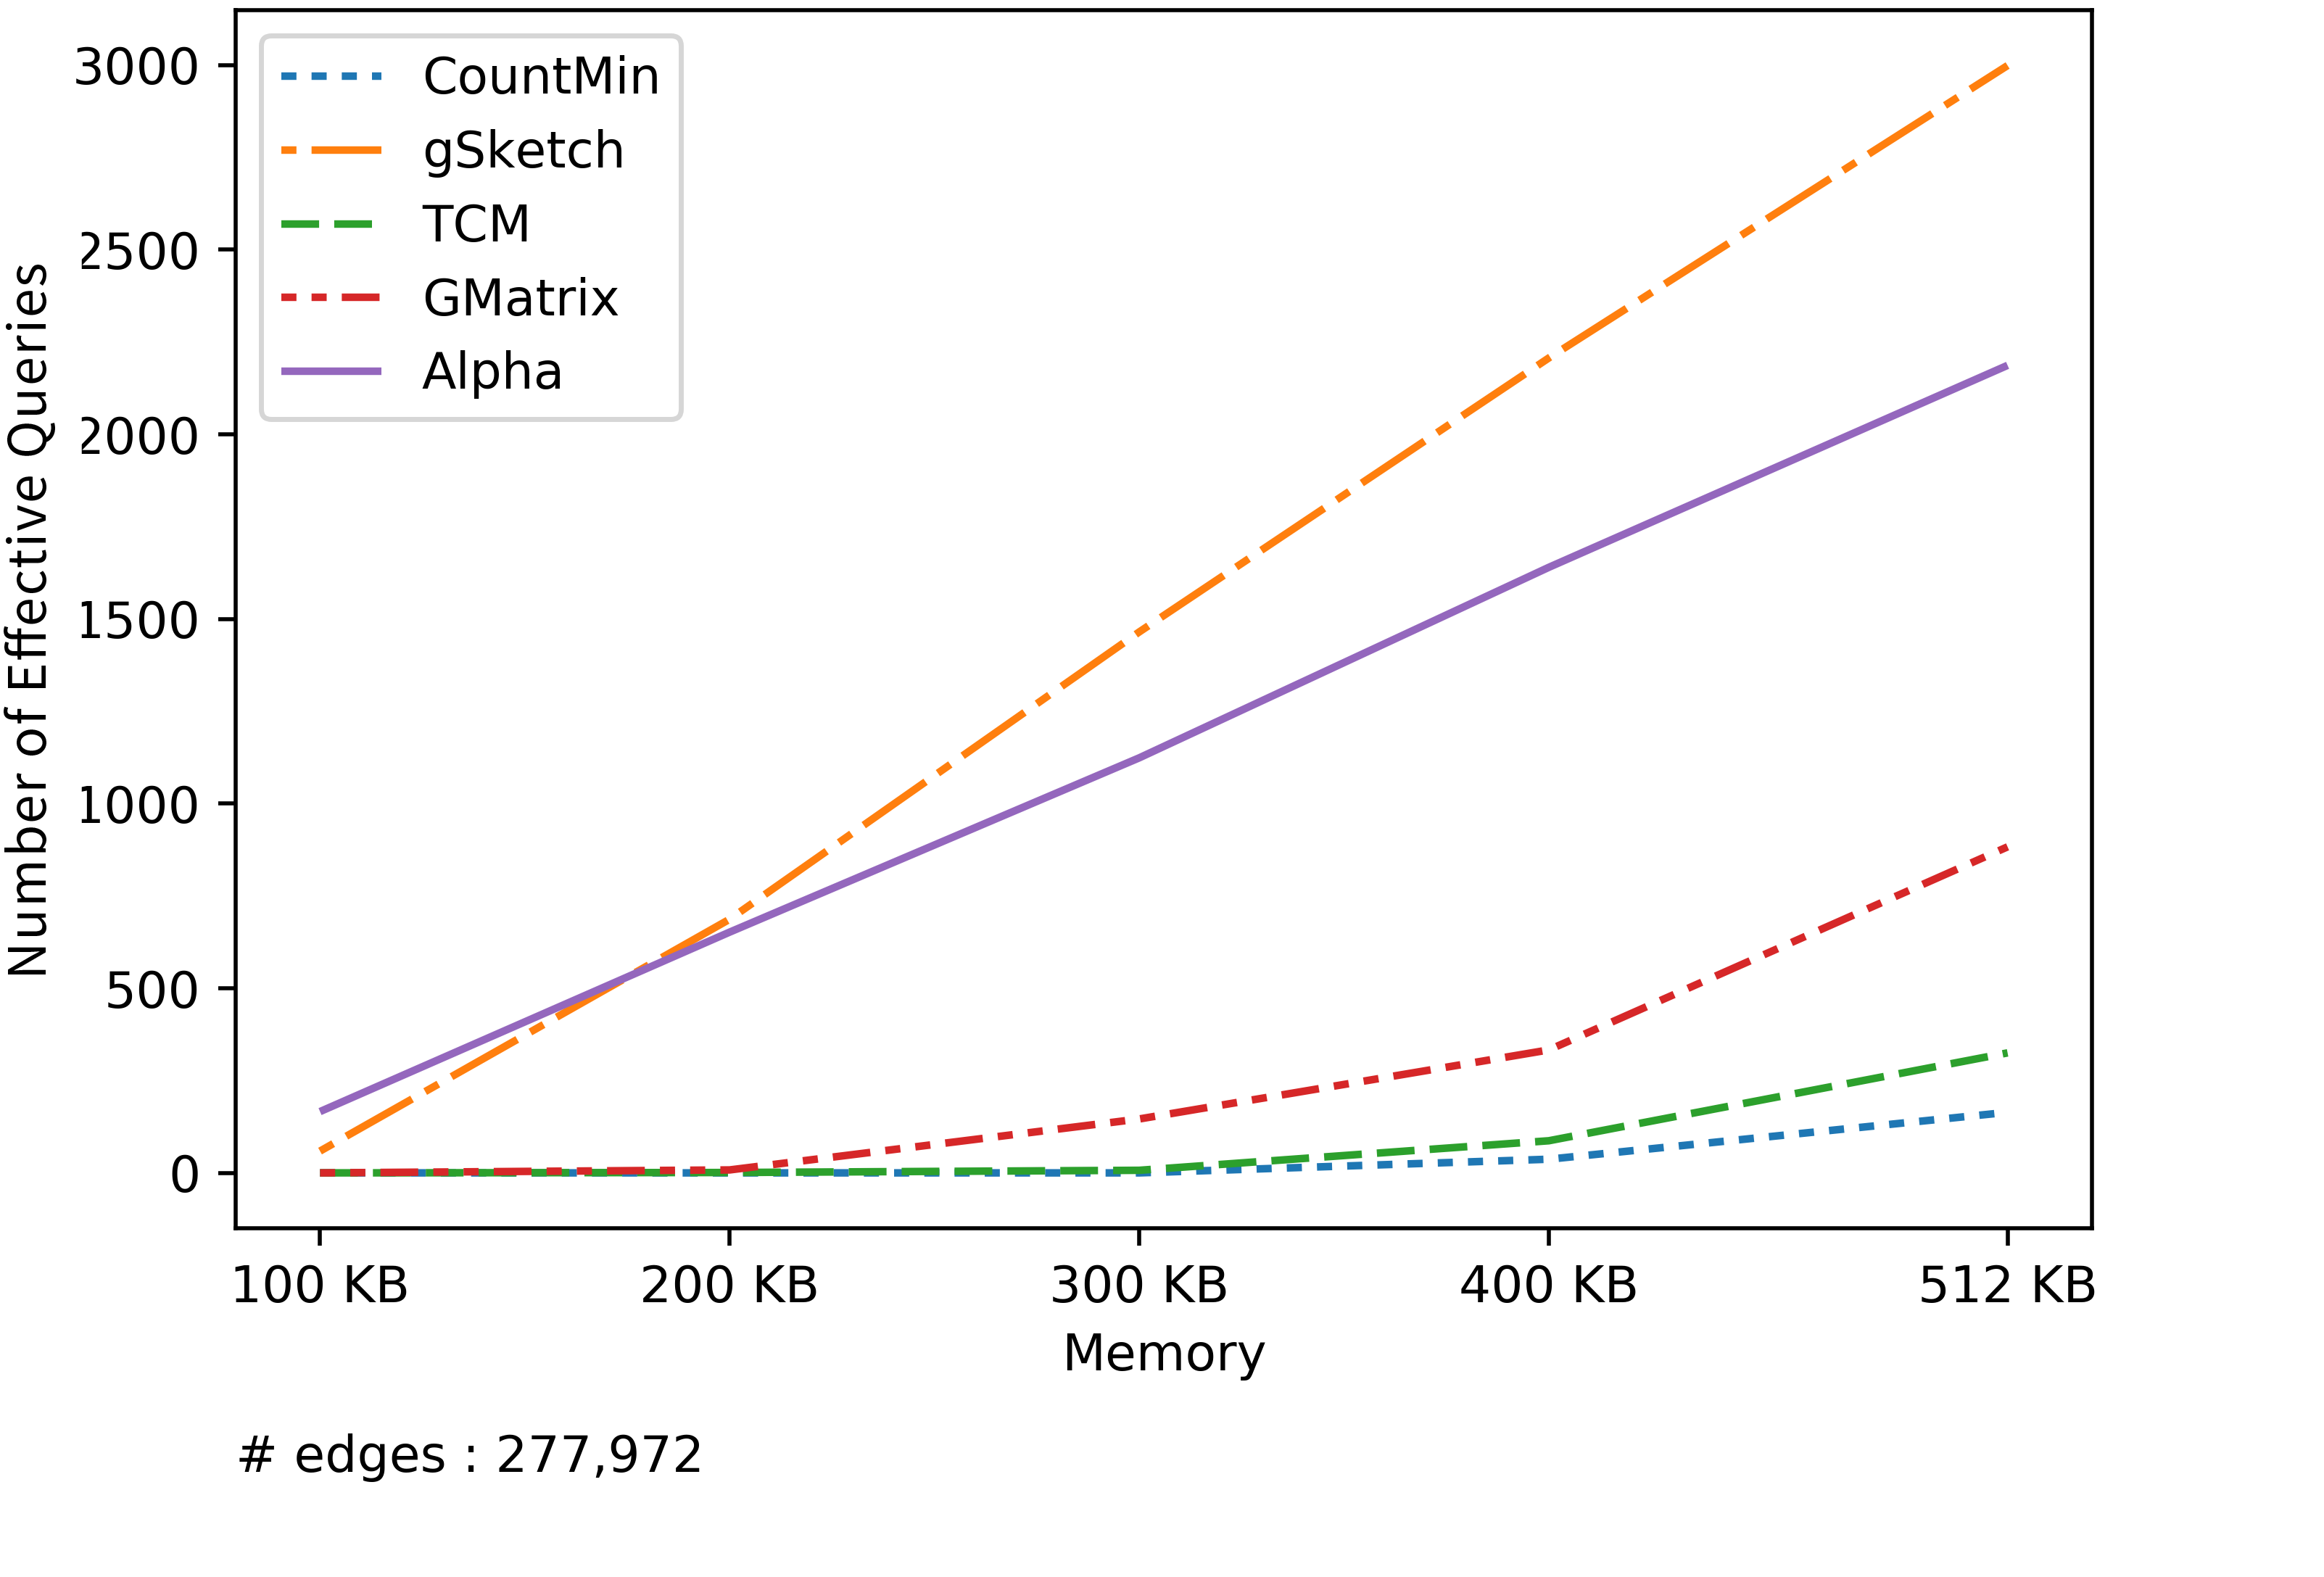
\includegraphics[width=0.85\textwidth]{results/neq/unicorn-wget-neq}
    \vspace{-0.5cm}
    \caption{Number of effective queries vs Memory for unicorn-wget dataset}
    \label{fig:unicorn-wget-neq}
\end{figure}

\begin{figure}[H]
    \centering 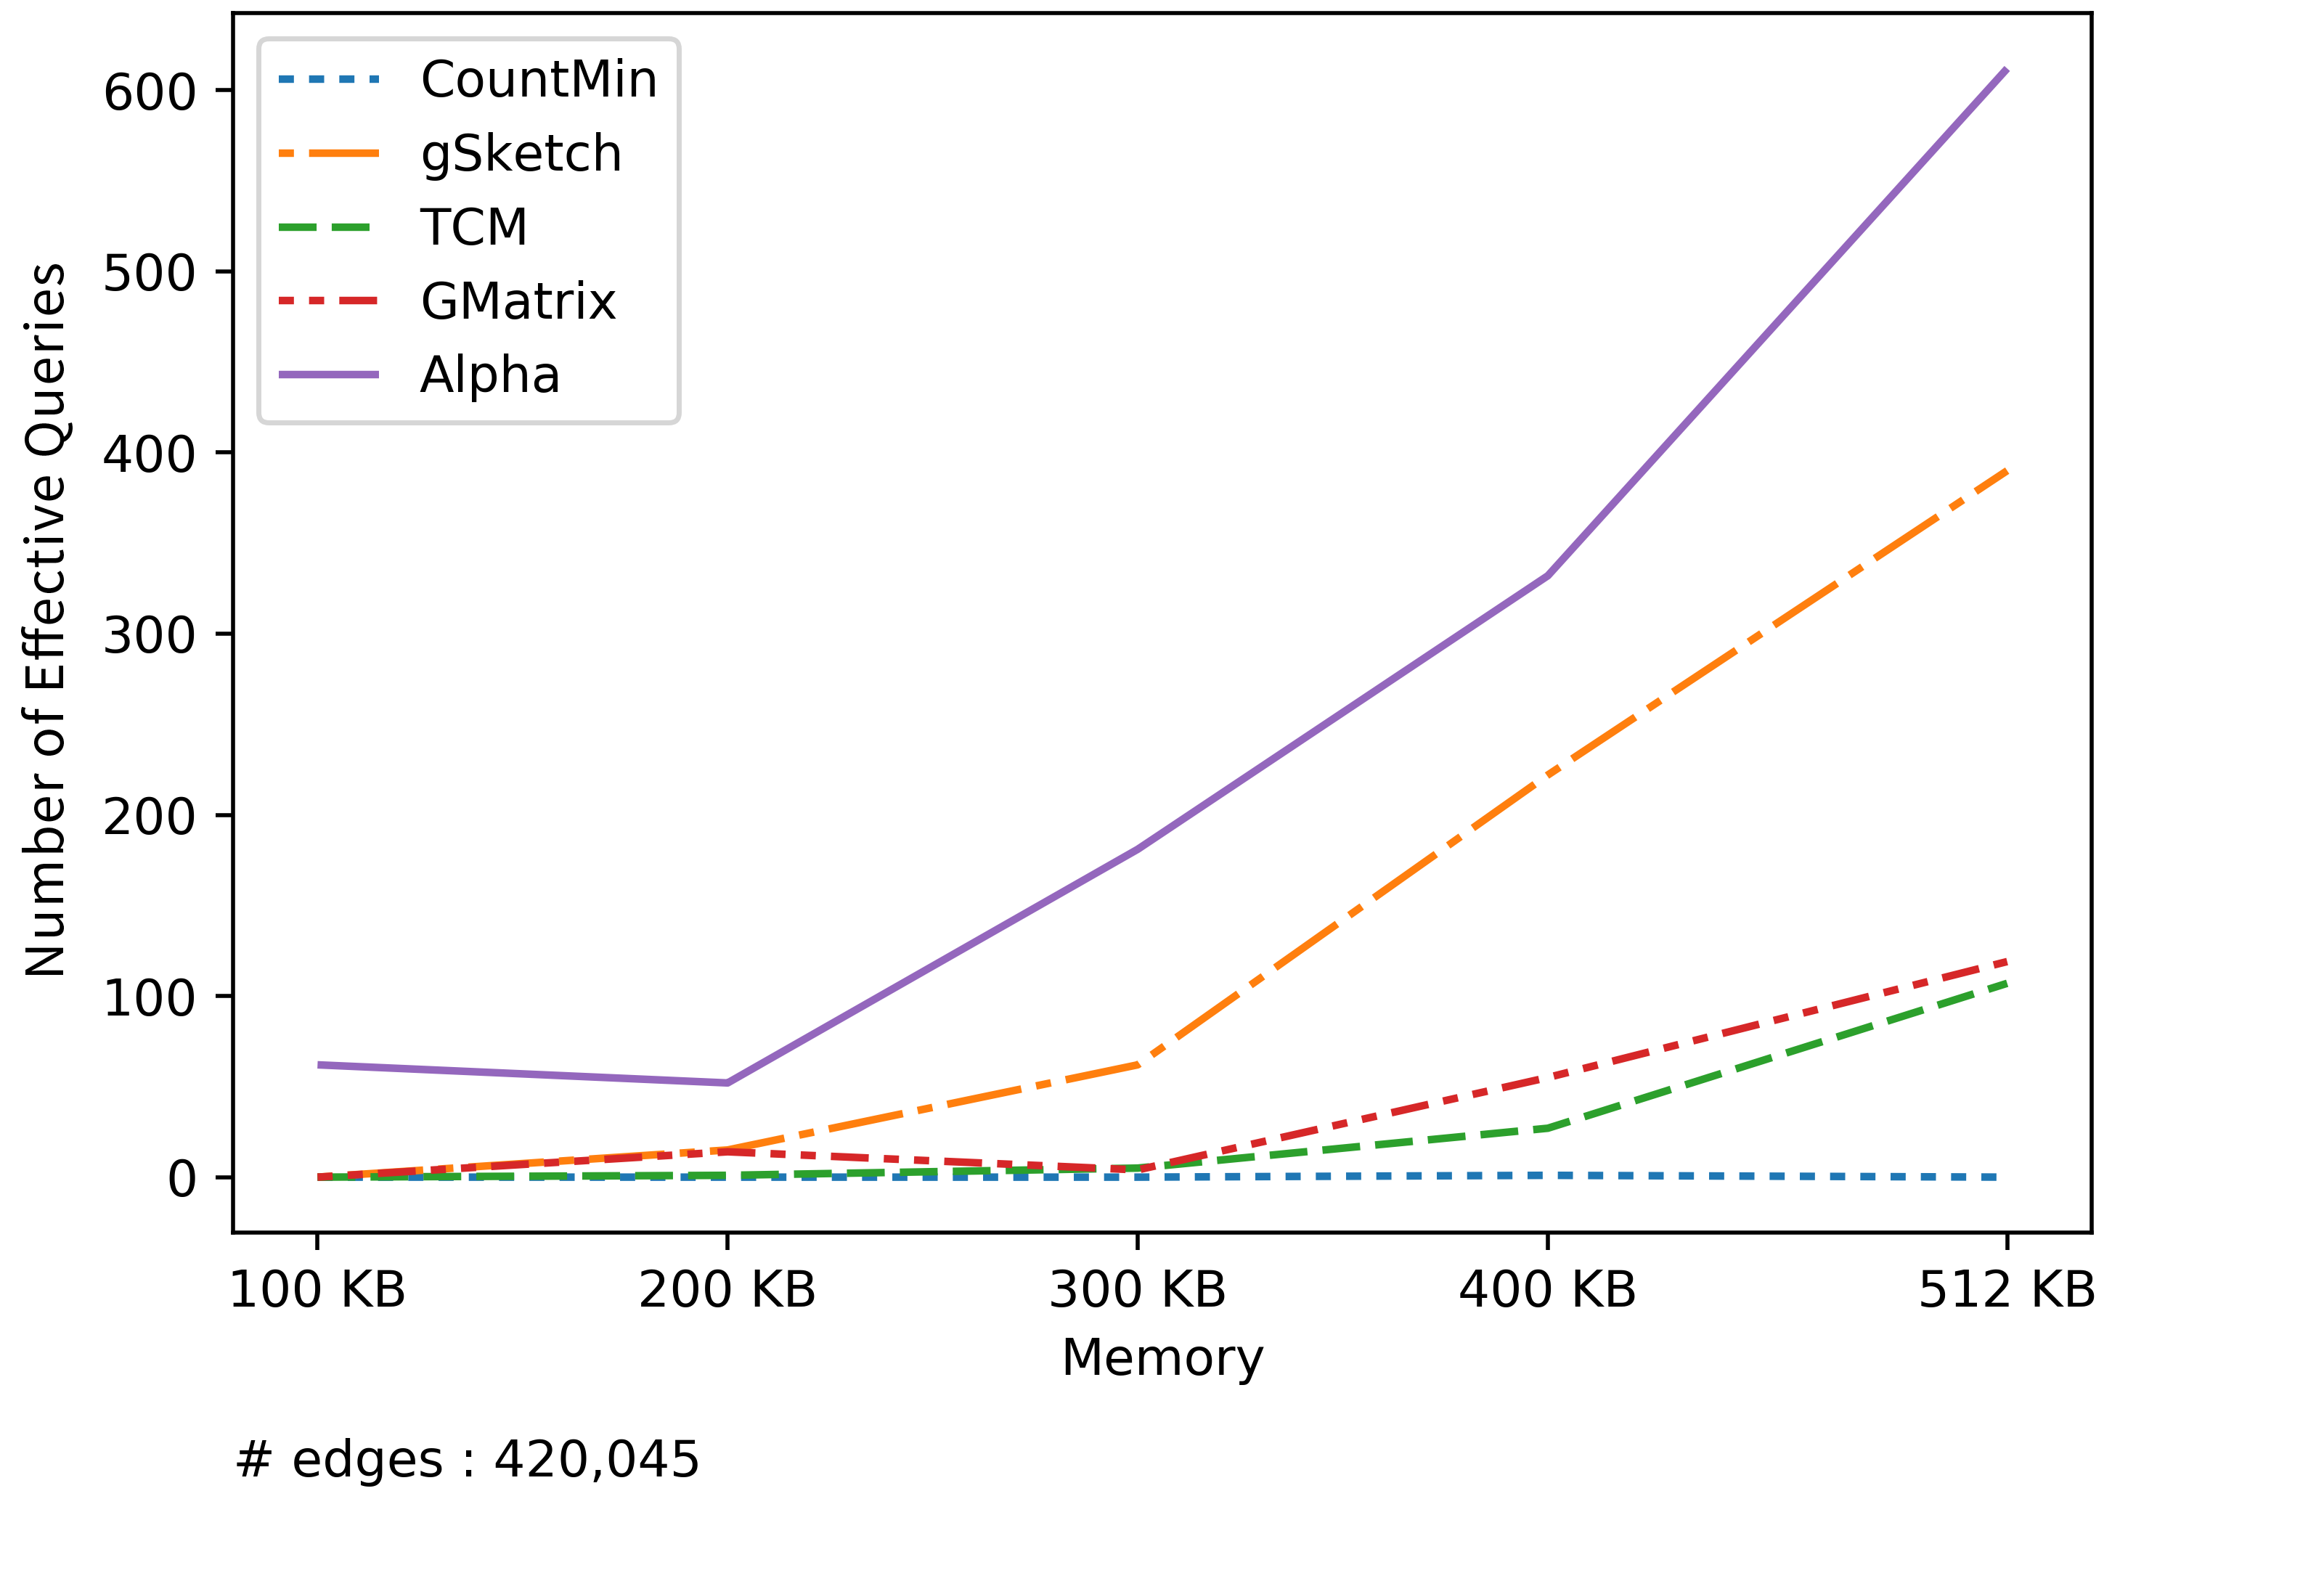
\includegraphics[width=0.85\textwidth]{results/neq/email-EuAll-neq}
    \vspace{-0.5cm}
    \caption{Number of effective queries vs Memory for email-EuAll dataset}
    \label{fig:email-EuAll-neq}
\end{figure}

\begin{figure}[H]
    \centering 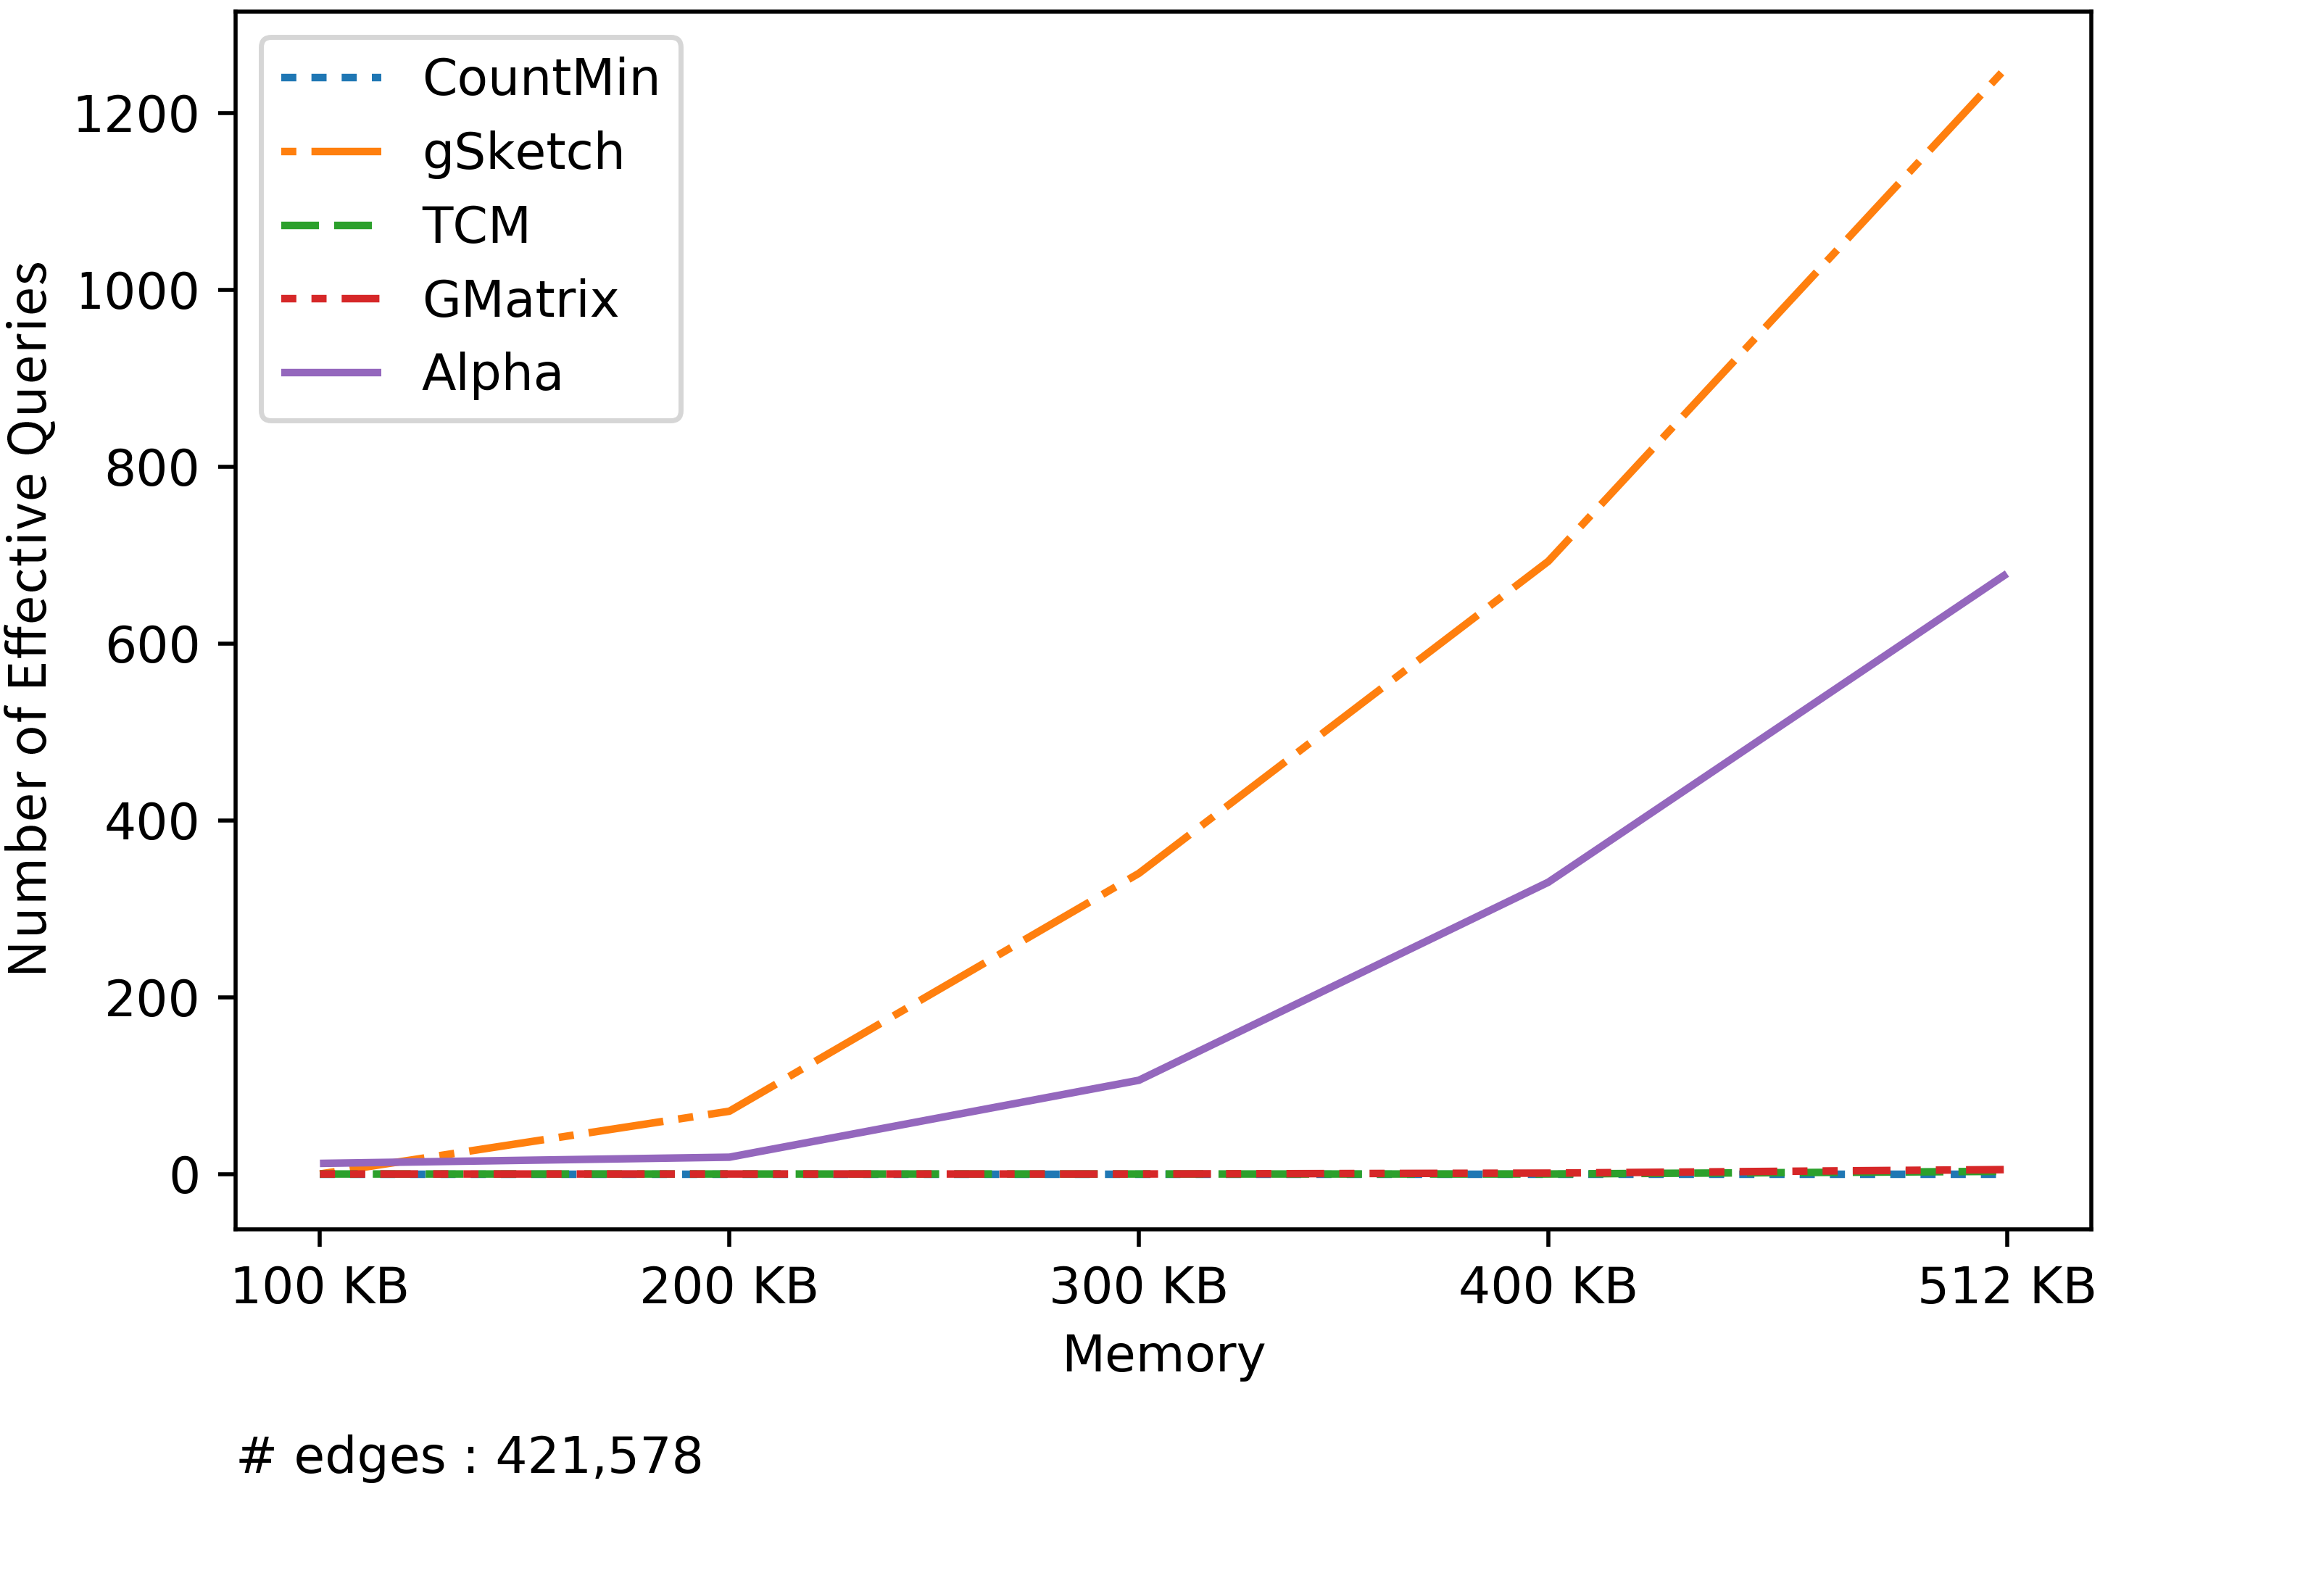
\includegraphics[width=0.85\textwidth]{results/neq/cit-HepPh-neq}
    \vspace{-0.5cm}
    \caption{Number of effective queries vs Memory for cit-HepPh dataset}
    \label{fig:cit-HepPh-neq}
\end{figure}

\begin{figure}[H]
    \centering 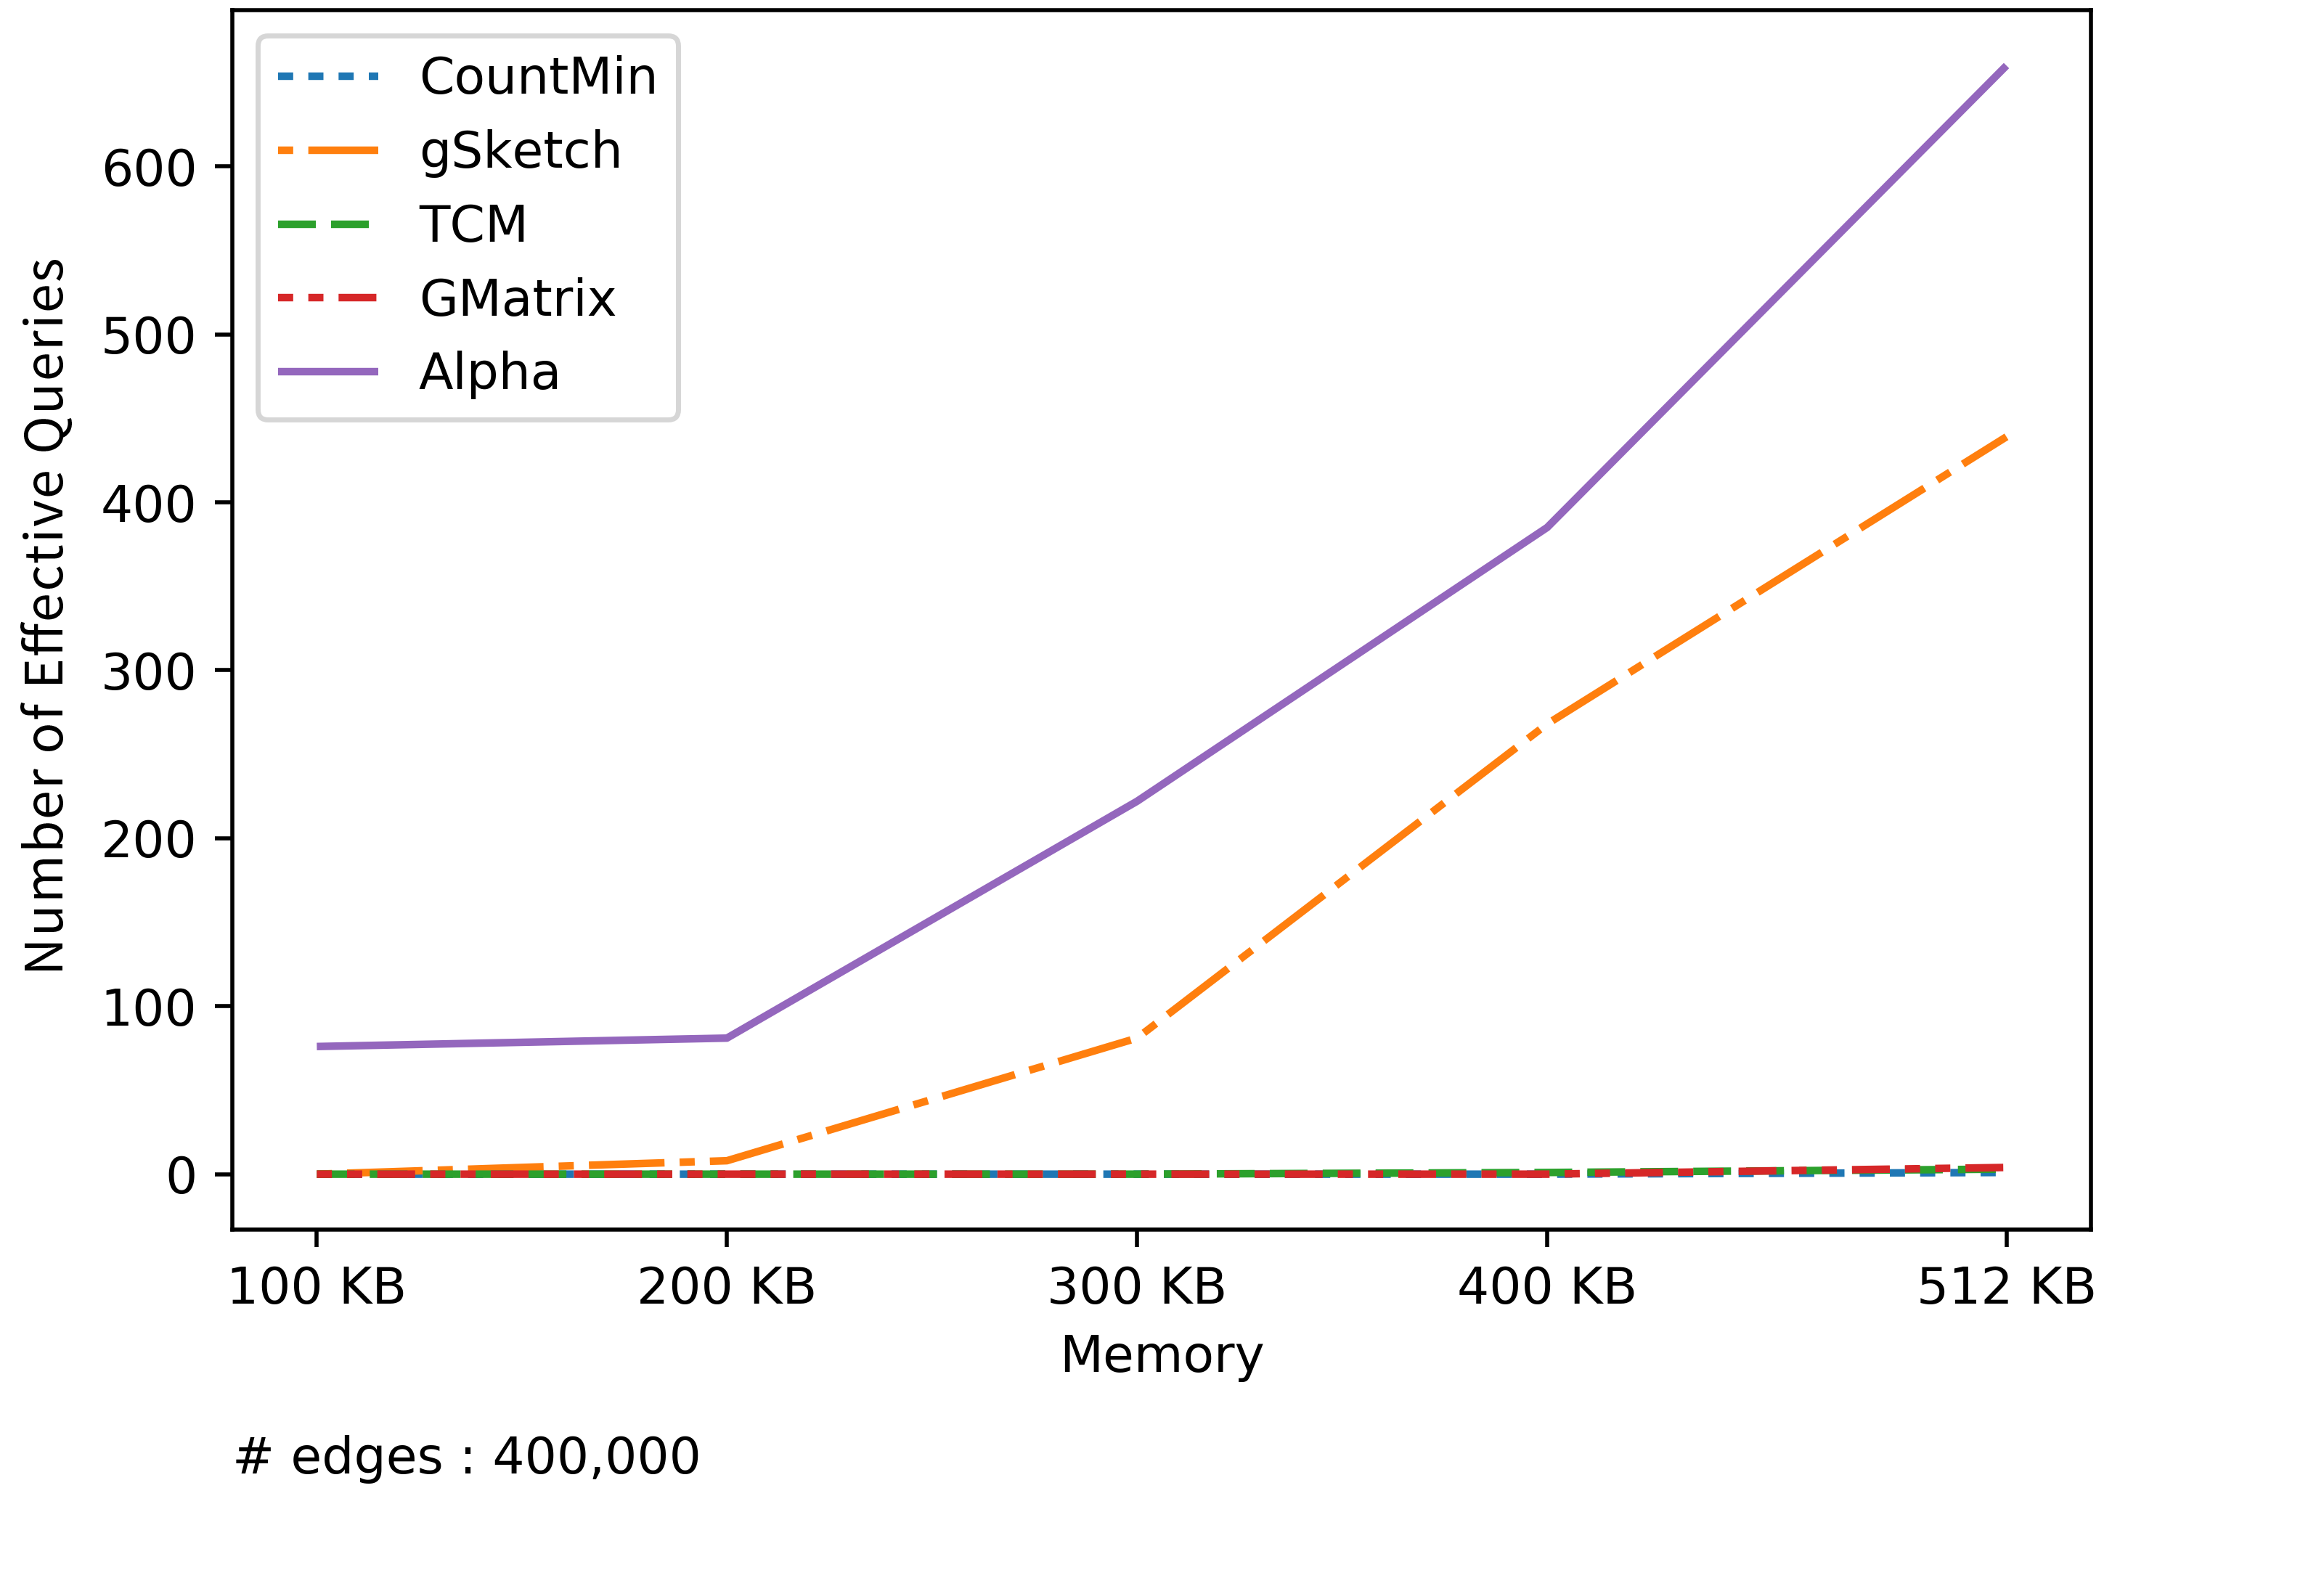
\includegraphics[width=0.85\textwidth]{results/neq/gen-scale-free-neq}
    \vspace{-0.5cm}
    \caption{Number of effective queries vs Memory for gen-scale-free dataset}
    \label{fig:gen-scale-free-neq}
\end{figure}

\begin{figure}[H]
    \centering 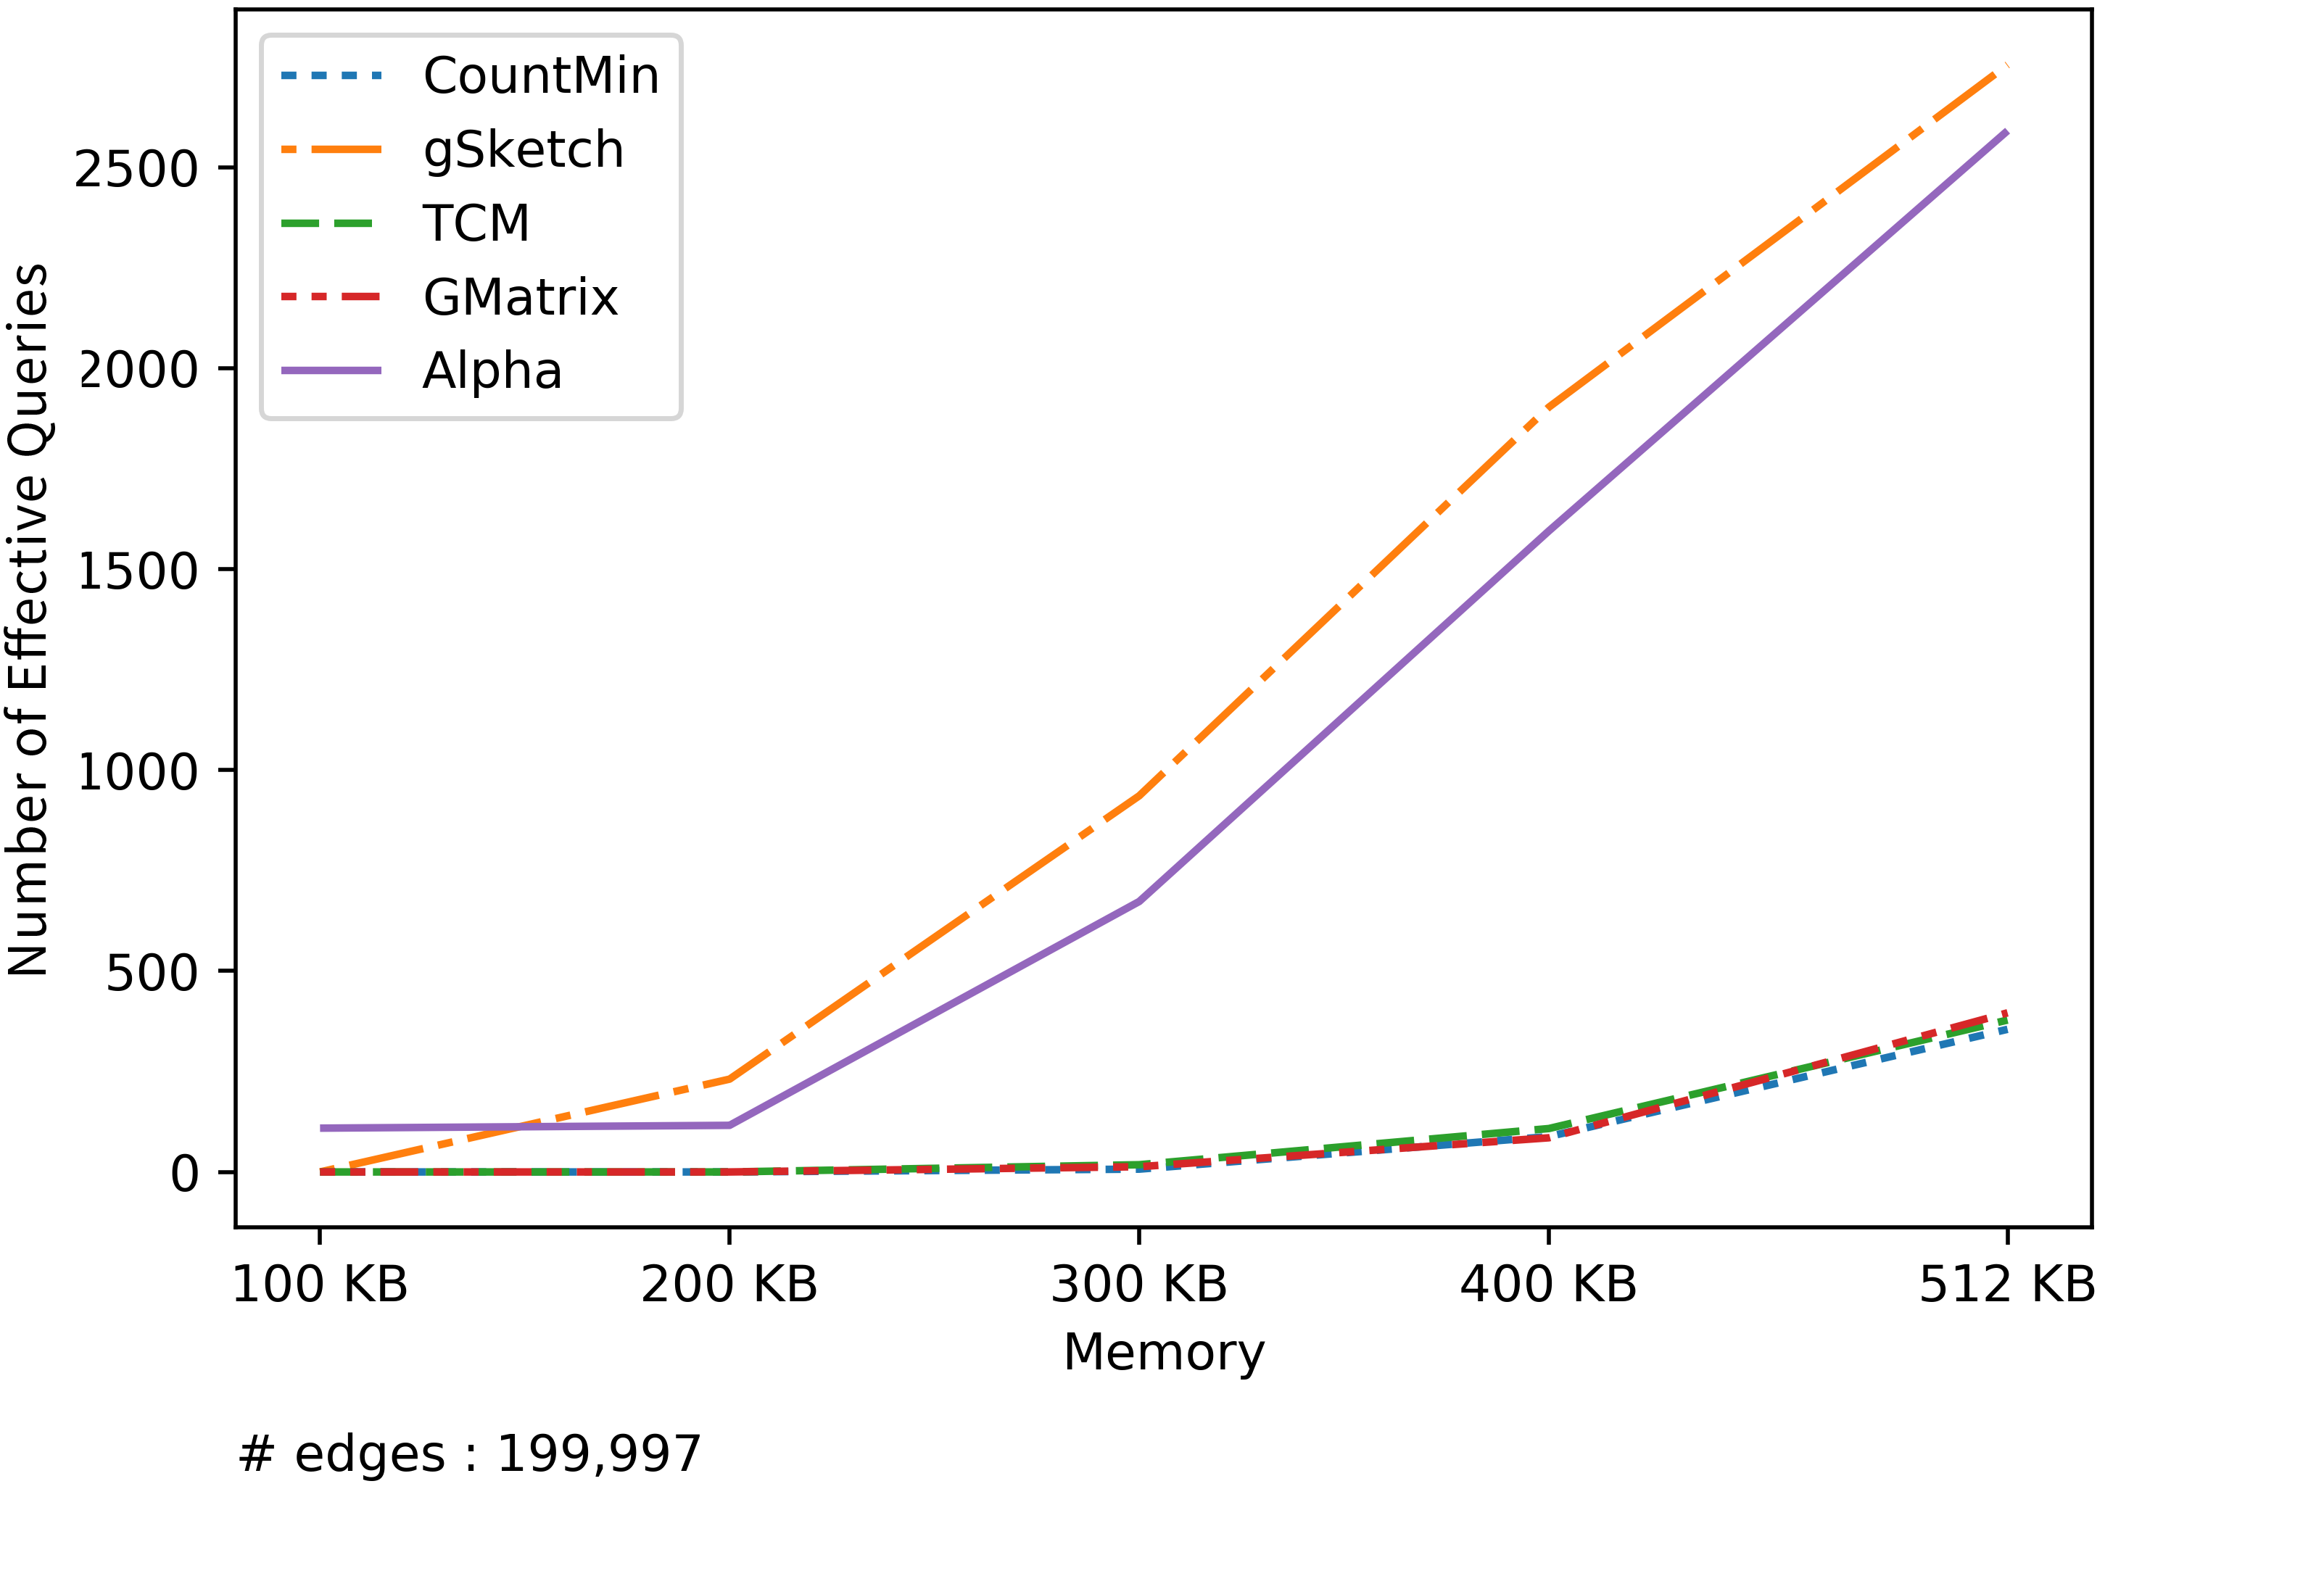
\includegraphics[width=0.85\textwidth]{results/neq/gen-small-world-neq}
    \vspace{-0.5cm}
    \caption{Number of effective queries vs Memory for gen-small-world dataset}
    \label{fig:gen-small-world-neq}
\end{figure}

\subsection*{Observations and inferences}

\paragraph{}
The number of effective queries for each sketch was calculated by querying the sketches against 10,000 edges, which were chosen through reservoir sampling from the original dataset. 

\paragraph{}
In the results for the datasets, unicorn-wget in \autoref{fig:unicorn-wget-neq}, cit-HepPh in \autoref{fig:cit-HepPh-neq} and gen-small-world in \autoref{fig:gen-small-world-neq}; Alpha has a significantly higher number of effective queries in general than all the other sketches except for gSketch.

\paragraph{}
Alpha has surpassed the accuracy of gSketch for email-EuAll in \autoref{fig:email-EuAll-neq} and gen-scale-free in \autoref{fig:gen-scale-free-neq}. 

\paragraph{}
All the sketches for the tested datasets have produced poor accuracies. The unicorn-wget dataset shows the highest number of effective queries for the tested datasets. However, even that result has capped around 3,000 effective queries per 10,000 queries in total. It can be inferred that the low accuracy for the datasets has been a result of the higher compression ratio. It is possible to achieve a better accuracy through allocation of more memory for the sketches. 

\paragraph{}
Alpha has a much higher accuracy with regard to number of effective queries in comparison to TCM, GMatrix and CountMin. This is sufficient to prove the superiority of the proposed solution against the existing sketching techniques. 